%=======================================================================
%  LABORATORIO N.o 2 - DIODOS: CURVA CARACTERISTICA
%  Curso : Circuitos Electronicos  (2026-2)
%  UCSP  - Facultad de Ingenieria - Ing. Electronica y de Telecomunicaciones
%  Docente     : Ebert San Roman Castillo
%  Laboratorio : Ing. Jeanpier Ancori Sanchez
%
%  Version 2 - Fusion de dos guias de origen:
%
%    (B) "Lab. 01 - v2026-1 - Diodo - Curva Caracteristica.doc"
%        Aporta la ESTRUCTURA y todo el procedimiento calificado
%        (secciones I, III, IV, V, VI, VII, VIII y los temas de II.3).
%
%    (A) "Laboratorio_2_Propedeucio EEB.doc"
%        Aporta unicamente la teoria del diodo (II.1), de la que (B) carece.
%
%  Por decision del autor NO se incorpora el resto de (A): osciloscopio,
%  generador de senales, rectificacion de senales y las actividades con la
%  Electronics Explorer Board. Esa transcripcion completa e independiente
%  queda en  Laboratorio_2_v1_rectificacion.tex,  que sigue compilando.
%
%  No se anade contenido propio. Sobre los originales solo se hizo:
%    - Corregir erratas evidentes ("se parecia" -> "se aprecia",
%      "pareciar" -> "apreciar", "en le Diodo" -> "en el Diodo",
%      "esta conectado" -> "este conectado").
%    - Sustituir los objetos de Editor de ecuaciones de (B) -- que en el
%      .doc eran imagenes .wmf sueltas -- por matematicas nativas:
%      image2=uA, image4/image10=V1, image5/image7=V2, image11=VD,
%      image6/image8/image12=ID, image14="VD vs ID".
%    - Dejar que LaTeX numere secciones, figuras y tablas. El original (B)
%      repite el numeral "V." en dos secciones seguidas y (A) repite el
%      numero de figura 10; con \ref eso se corrige solo.
%    - Reemplazar la portada y el membrete de (B), que eran imagenes
%      escaneadas, por la cabecera que construye este mismo archivo.
%
%  Version 3 - La practica trata del diodo en polarizacion directa e inversa,
%  asi que se retira la teoria del condensador (antigua II.2, procedente de (A)
%  y ajena al tema) con sus seis figuras. El resto del documento no cambia: la
%  seccion era autocontenida y ninguna otra la referenciaba. La lista de
%  materiales de (B) nunca incluyo condensadores, por lo que queda intacta.
%
%  El preambulo se alinea con el del Laboratorio 1 para que ambas guias se vean
%  iguales: misma geometria de pagina (bottom=2.6cm, footskip=1.2cm) y pie de
%  una sola linea. Unicos anadidos propios de esta guia: \puntos, que rotula el
%  peso de cada seccion calificada, y \tablename -> "Tabla", porque el texto
%  dice "la tabla 1" y babel-spanish rotularia "Cuadro 1".
%
%  Version 4 - Se anade la seccion VI, "Ejercicio adicional: el diodo como
%  capacitor variable", que no procede de ninguna de las dos guias. Prolonga la
%  polarizacion inversa (IV.2): el diodo en inversa presenta una capacitancia de
%  juntura que, con L1, forma un resonador sintonizable por tension.
%    - circuito_resonador.png  es el esquema del simulador.
%    - bode_resonador.pdf      lo genera herramientas/graficar_bode.py leyendo
%                              LAB2.DAT, el barrido en alterna exportado por el
%                              simulador. Va en PDF, no en PNG: una curva es
%                              vectorial y asi no pixela ni engorda el archivo.
%  Esta seccion todavia NO tiene puntaje asignado; las demas suman ya los 20.
%
%  Version 5 - Se pone al dia "Equipos y materiales", que habia quedado como
%  estaba en (B) pese a los anadidos de la version 4:
%    - Software: se admite Multisim o Proteus (la lista decia uno y el
%      procedimiento pedia el otro) y se anade Python, que la guia exige en la
%      seccion VI.3 y en el analisis de resultados pero no aparecia por ningun
%      lado.
%    - Los componentes del resonador (L1, C1, R1, R2, V2) NO se anaden a los
%      fungibles: esa seccion es solo de simulador y no hay nada que comprar.
%      En su lugar se abre la seccion VI con una nota que los enumera y lo
%      deja dicho.
%
%  Version 6 - Se rehacen las dos tablas de lecturas para que la practica se
%  pueda hacer con la Analog Discovery Studio, cuya fuente no llega a los 30 V
%  que pedia la guia original (tiene fuentes programables de 1 a 5 V, railes
%  fijos de 12/5/3,3 V y un generador W1 de +-5 V).
%    - Tabla 1 (directa): de 18 a 13 lecturas, ahora 0,2..10 V. Las ocho
%      primeras cubren el codo (0,2 a 1,0 V), donde V_D va de 199 a 529 mV; las
%      cinco ultimas (2, 4, 6, 8 y 10 V) el tramo saturado, donde V_D apenas
%      sube de 583 a 683 mV. El recorte no es solo instrumental: a 30 V
%      circulaban 29 mA y R1, de 0,25 W, disipaba 0,86 W.
%    - Tabla 2 (inversa): de 10 a 13 lecturas, con exactamente los mismos
%      valores de V1 que la tabla 1, de modo que la curva conjunta del
%      analisis de resultados quede simetrica respecto al origen.
%    - La guia no dice que salida del ADS corresponde a cada tramo: se decidio
%      dejar las tablas solas, sin nota de instrumentacion.
%
%    - A image22.png (figura 5) se le quito el marco discontinuo del simulador
%      y el widget de zoom que lo acompanaba, para que la figura quede como la
%      del circuito de directa (image21.png): solo el esquema, sin cromo de la
%      aplicacion. La captura sin retocar sigue en image22_original.png.
%
%  Version 7 - La seccion VI deja de ser un "ejercicio adicional" de simulador y
%  pasa a montarse tambien en protoboard, con estas consecuencias:
%    - Se le quita el rotulo "Ejercicio adicional" al titulo y se le pone la
%      etiqueta sec:varicap, para poder referenciarla desde los materiales.
%    - Se elimina la nota tecnica que decia que el apartado no se montaba y que
%      por eso sus componentes no estaban en la lista. De paso desaparece un
%      error suyo: afirmaba que D1 era el 1N4007, cuando la figura del circuito
%      y las preguntas 1 y 5 hablan del 1N4149.
%    - Sus componentes pasan a "Equipos y materiales": el 1N4149, R2 de 100 k,
%      C1 de 10 uF, el condensador de 1 nF con que se verifica la bobina, y el
%      alambre y el formador con que se construye L1. R1 de 1 k ya estaba
%      cubierto por las 6 unidades que pedia la lista.
%    - Se anade el apartado VI.2, "Construccion del inductor L1": L1 no se
%      compra, se bobina. Solenoide de una capa con nucleo de aire porque asi el
%      valor sale de la geometria y se puede calcular. Lleva la formula de
%      Wheeler en mm, el despeje completo de N (queda una cuadratica: 59 vueltas
%      sobre formador de 10 mm, 33,6 mm de largo, 2,2 m de alambre), la
%      justificacion del calibre AWG 24 por efecto pelicular (a 30 MHz solo
%      conducen 12 um de los 255 um de radio) y una verificacion por resonancia
%      con el condensador de 1 nF, que cae en 1,59 MHz y si es medible.
%    - Se anade un paso d) al procedimiento: el barrido en alterna esta por
%      encima de los 30 MHz y el instrumental no llega, asi que sobre el montaje
%      real se mide la polarizacion continua del diodo, que si se puede.
%
%  PENDIENTE: la seccion VI sigue sin puntaje. Las demas suman ya los 20 puntos,
%  asi que darselo obliga a redistribuir; queda a criterio del docente.
%
%  Imagenes: image03-image05 provienen de (A); image21-image23 de (B).
%  Las image06-image11 (condensador) quedan en imagenes/ pero ya no se usan.
%  La figura 1 de (B) venia en EMF vectorial y se rasterizo a 2094 px.
%
%  Compilar:  xelatex Laboratorio_2.tex    (dos veces)
%=======================================================================
\documentclass[11pt,a4paper]{article}

%------------------------------------------------------------- idioma
% Compilar con XeLaTeX (no con pdflatex): Trebuchet MS es una fuente TrueType
% del sistema y solo fontspec, bajo XeLaTeX o LuaLaTeX, sabe cargarla.
% inputenc y fontenc se omiten a proposito: XeLaTeX trabaja en UTF-8 de forma
% nativa y esos paquetes dan error con este motor.
\usepackage{fontspec}
\setmainfont{Trebuchet MS}[
  Path            = C:/Windows/Fonts/,
  Extension       = .ttf,
  UprightFont     = trebuc,
  BoldFont        = trebucbd,
  ItalicFont      = trebucit,
  BoldItalicFont  = trebucbi,
  Ligatures       = TeX
]
\usepackage[spanish,es-nodecimaldot]{babel}
\usepackage{microtype}

%----------------------------------------------------------- geometria
\usepackage[left=2.4cm,right=2.4cm,top=3.1cm,bottom=2.6cm,headheight=30pt,
            footskip=1.2cm]{geometry}

%------------------------------------------------------------ graficos
\usepackage{graphicx}
\usepackage{float}
\usepackage{placeins}
\usepackage[font=small,labelfont=bf,labelsep=period]{caption}
\graphicspath{{imagenes/}}

%-------------------------------------------------------------- tablas
\usepackage{array}
\usepackage{tabularx}
\usepackage{booktabs}
\usepackage{multirow}

%----------------------------------------------------- matematicas / SI
\usepackage{amsmath,amssymb}
\usepackage{siunitx}
\sisetup{
  output-decimal-marker = {,},
  per-mode              = symbol,
  range-phrase          = { a },
  range-units           = single,
  detect-weight         = true,
  detect-family         = true
}

%--------------------------------------------------------------- listas
\usepackage{enumitem}
\setlist[itemize]{itemsep=3pt,topsep=4pt,parsep=0pt}
\setlist[enumerate]{itemsep=8pt,topsep=4pt,parsep=0pt}

%--------------------------------------------------------------- cajas
\usepackage[most]{tcolorbox}
\usepackage{pgffor}

\newtcolorbox{notatec}[1]{enhanced,breakable,
  colback=blue!3!white, colframe=blue!55!black,
  fonttitle=\bfseries\small, title={Nota técnica --- #1},
  boxrule=0.6pt, arc=2pt, left=6pt,right=6pt,top=4pt,bottom=4pt}

\newtcolorbox{seguridad}[1]{enhanced,breakable,
  colback=red!3!white, colframe=red!60!black,
  fonttitle=\bfseries\small, title={Seguridad --- #1},
  boxrule=0.6pt, arc=2pt, left=6pt,right=6pt,top=4pt,bottom=4pt}

\newtcolorbox{ejemplo}[1]{enhanced,breakable,
  colback=green!3!white, colframe=green!45!black,
  fonttitle=\bfseries\small, title={Ejemplo de diseño --- #1},
  boxrule=0.6pt, arc=2pt, left=6pt,right=6pt,top=4pt,bottom=4pt}

%------------------------------------------------------------ comandos
% Lineas punteadas para respuestas del alumno: \lineasresp{n}
\newcommand{\lineasresp}[1]{%
  \par\vspace{6pt}%
  \foreach \i in {1,...,#1}{\noindent\rule{\linewidth}{0.4pt}\par\vspace{11pt}}%
}

% Puntaje al final del titulo de una seccion calificada.
\newcommand{\puntos}[1]{\normalfont\normalsize\textmd{(#1 puntos)}}

%---------------------------------------------------- encabezado / pie
\usepackage{fancyhdr}
\pagestyle{fancy}
\fancyhf{}
\fancyhead[L]{\footnotesize UCSP --- Facultad de Ingeniería\\
              Ing. Electrónica y de Telecomunicaciones}
\fancyhead[R]{\footnotesize 2026-2 Circuitos Electrónicos\\
              Ebert San Román Castillo}
\fancyfoot[L]{\footnotesize Laboratorio N.\textsuperscript{o} 2 --- Diodos: curvas características y capacitancia del diodo}
\fancyfoot[R]{\footnotesize Página \thepage\ de \pageref{LastPage}}
\renewcommand{\headrulewidth}{0.4pt}
\renewcommand{\footrulewidth}{0.4pt}
\usepackage{lastpage}

%------------------------------------------------------- numeracion
\renewcommand{\thesection}{\Roman{section}}
\renewcommand{\thesubsection}{\arabic{subsection}}

%-------------------------------------------------------- hiperenlaces
\usepackage[hidelinks,pdfusetitle]{hyperref}
\hypersetup{
  pdftitle={Laboratorio 2 - Diodos: curvas caracteristicas y capacitancia del diodo},
  pdfsubject={Circuitos Electronicos - Guia de practicas},
  pdfauthor={Ebert San Roman Castillo; Jeanpier Ancori Sanchez},
  pdfkeywords={electronica, diodo, 1N4007, 1N4149, curvas caracteristicas,
               polarizacion directa, polarizacion inversa, capacitancia de juntura,
               varicap, resonador LC, Multisim}
}

% babel-spanish rotula las tablas como "Cuadro"; los originales dicen "Tabla"
% y asi lo pide el texto de la guia ("las medidas solicitadas en la tabla 1").
\addto\captionsspanish{\renewcommand{\tablename}{Tabla}}

\begin{document}

%=======================================================================
%  CABECERA DE LA GUIA
%=======================================================================
% El documento es de 11 pt, asi que \normalsize son los 11 pt del Word original.
\begin{center}
    {\normalsize\bfseries PRIMERA UNIDAD: DIODOS Y APLICACIONES BÁSICAS}
\end{center}

\vspace{0.55cm}

% Cabecera identica a la del Laboratorio 1 (ver los comentarios de aquel archivo).
% Sustituye a la portada escaneada del .doc de origen.
\begingroup
\renewcommand{\tabularxcolumn}[1]{m{#1}}
\renewcommand{\arraystretch}{2.0}
\setlength{\tabcolsep}{12pt}
\noindent
\begin{tabularx}{\textwidth}{|>{\centering\arraybackslash}m{2.2cm}|>{\centering\arraybackslash}X|>{\centering\arraybackslash}m{3.0cm}|}
\hline
\rule{0pt}{2.1cm}{\fontsize{58}{58}\selectfont\bfseries 2}
    & \begin{minipage}[c]{\linewidth}\centering
          {\large\bfseries Guía de Prácticas}\\[7pt]
          {\Large\bfseries Diodos --- Curvas Características\\ y Capacitancia del Diodo}
      \end{minipage}
    & {\Large\bfseries Nota}\\
\hline
\multicolumn{3}{|l|}{\rule{0pt}{1.3cm}\large\textbf{Grupo:}~\rule{4.6cm}{0.4pt}%
    \hfill\large\textbf{Fecha:}~\rule{4.6cm}{0.4pt}\hspace{2mm}}\\
\hline
\multicolumn{3}{|l|}{\rule{0pt}{1.2cm}\large\textbf{Alumno(s):}~\rule{11.2cm}{0.4pt}\hspace{2mm}}\\
\multicolumn{3}{|l|}{\rule{0pt}{1.2cm}\phantom{\large\textbf{Alumno(s):}}~\rule{11.2cm}{0.4pt}\hspace{2mm}}\\
\hline
\end{tabularx}
\endgroup

\vspace{1.2cm}

%=======================================================================
\section{Objetivos}
%=======================================================================
El objetivo principal de esta práctica es conocer experimentalmente la operación del diodo
semiconductor, para lo cual se desarrollan las siguientes actividades:

\begin{itemize}
    \item Polarización del diodo en forma directa, a fin de representar su curva característica
          de operación.
    \item Polarización del diodo en forma inversa, a fin de representar su curva característica
          de operación.
    \item Análisis del comportamiento externo del diodo semiconductor en sus diferentes
          polarizaciones.
    % Objetivo anadido junto con el titulo: este cubre la seccion VI, que hasta
    % ahora no estaba representada en la lista.
    \item Medición de la capacitancia de juntura del diodo en polarización inversa y su
          empleo como capacitor variable en un resonador $LC$.
\end{itemize}

%=======================================================================
\section{Contenido teórico}
%=======================================================================
\subsection{El diodo}

Los semiconductores han revolucionado el mundo de la electrónica y han permitido grandes avances
en casi todas las ciencias; el más simple de los semiconductores es el diodo. El diodo solo
permite la circulación de la corriente en un único sentido, como se aprecia en la
figura~\ref{fig:diodo-func}, donde en la primera configuración permite el paso de corriente y en
la segunda la evita, principio del rectificador.

\begin{figure}[H]
    \centering
    
\includegraphics[width=0.75\textwidth]{image03.png}
    \caption{Funcionamiento del diodo.}
    \label{fig:diodo-func}
\end{figure}

Los semiconductores son elementos que en condiciones normales son aislantes, pero con cierta
modificación en su organización molecular pueden convertirse en conductores. Esta modificación
consiste básicamente en el dopado con otros elementos que poseen enlaces covalentes incompletos;
ejemplos de semiconductores son el silicio, el selenio y el germanio. El símbolo del diodo y el
dispositivo se pueden apreciar en la figura~\ref{fig:diodo-simb}.

\begin{figure}[H]
    \centering
    
\includegraphics[width=0.46\textwidth]{image04.png}
    \caption{Imagen y símbolo del diodo.}
    \label{fig:diodo-simb}
\end{figure}

El diodo está compuesto por la unión de un cristal tipo P con otro tipo N, en donde las cargas
opuestas de la unión AB crean una pequeña barrera de oposición, que con una mínima tensión de
polarización entre \qtyrange{0.2}{0.7}{\volt} logra la conducción de corriente en el diodo.

\begin{figure}[H]
    \centering
    
\includegraphics[width=0.95\textwidth]{image05.png}
    \caption{Esquema eléctrico del funcionamiento del diodo.}
    \label{fig:diodo-pn}
\end{figure}

\FloatBarrier
\subsection{Operación del diodo semiconductor y análisis de circuitos}

\begin{itemize}
    \item Operación interna del diodo semiconductor.
    \item Operación externa del diodo semiconductor.
    \item Análisis de circuitos con diodos: modelos de circuito equivalente para el diodo y
          análisis rápido de circuitos con diodos.
\end{itemize}

\FloatBarrier
%=======================================================================
\section{Equipos y materiales}
%=======================================================================
\noindent\textbf{Equipos y dispositivos:}
\begin{itemize}
    \item Fuente regulada de voltaje (\qtyrange{0}{30}{\volt}).
\end{itemize}

\noindent\textbf{Software:}
\begin{itemize}
    % El procedimiento de IV.1 y IV.2 pedia "Proteus" mientras esta lista decia
    % "Multisim". El circuito es el mismo en ambos, asi que se admiten los dos.
    \item Simulador de circuitos: Multisim o Proteus.
    % La guia exige Python dos veces (seccion VI.3 y analisis de resultados) pero
    % el original no lo listaba.
    \item Python~3 con las bibliotecas \texttt{numpy} y \texttt{matplotlib}, para
          trazar las gráficas que se piden en el análisis de resultados.
\end{itemize}

\vspace{0.25cm}
\noindent\textbf{Materiales y fungibles} (deben ser adquiridos por los alumnos). Comprar cada uno
de los siguientes valores:
\begin{itemize}
    \item 04 diodos 1N4007.
    % El original dice "1/4 vatio"; se expresa como 0,25 W, igual que en el Laboratorio 1.
    \item 06 resistencias de \qty{1}{\kilo\ohm} (\qty{0.25}{\watt}).
    \item 02 diodos LED azules.
    \item 01 motor DC de \qty{12}{\volt} (pequeño).
    % --- Componentes de la seccion VI (el diodo como capacitor variable). Antes no
    % estaban en esta lista porque aquel apartado se resolvia solo en el simulador;
    % ahora tambien se monta en protoboard, asi que hay que comprarlos.
    \item 01 diodo 1N4149 o 1N4148, para la sección~\ref{sec:varicap}. \emph{No} sirve el
          1N4007 en su lugar (véase la pregunta 5 de esa sección).
    \item 01 resistencia de \qty{100}{\kilo\ohm} (\qty{0.25}{\watt}).
    \item 01 condensador electrolítico de \qty{10}{\micro\farad} (\qty{25}{\volt} o más).
    \item 01 condensador cerámico de \qty{1}{\nano\farad} con tolerancia del
          \qty{5}{\percent} o mejor, para verificar el inductor.
    % El alambre calculado son ~2,2 m; se piden 3 m para tener margen de sobra si hay
    % que rebobinar la primera bobina, que casi siempre queda mal.
    \item \qty{3}{\metre} de alambre de cobre esmaltado AWG~24 y un cilindro rígido de
          \qty{10}{\milli\metre} de diámetro que sirva de formador (un tubo de PVC, una
          broca o el cuerpo de un plumón), para bobinar $L_1$: el inductor no se compra,
          se construye siguiendo el apartado~\ref{sec:varicap}.\ref{sec:bobina}.
    \item Lija fina o cúter, para retirar el esmalte de las puntas del alambre.
    \item 01 protoboard.
    \item 01 multímetro.
    \item Cables conectores para protoboard.
    \item Mandil (obligatorio).
\end{itemize}

\FloatBarrier
%=======================================================================
\section{Procedimiento}
%=======================================================================
\subsection{Polarización directa \puntos{4}}

\begin{enumerate}[label=\textbf{\alph*)}, leftmargin=*, labelsep=0.6em]
\item Arme el circuito de la figura~\ref{fig:pol-directa} y, en el simulador, tome las
medidas solicitadas en la tabla~\ref{tab:directa}.

\item En el protoboard, arme el circuito de la figura~\ref{fig:pol-directa}. Antes de encender la
fuente de alimentación considere lo siguiente:
\end{enumerate}

\begin{itemize}
    \item Revisar que el ánodo del diodo esté conectado a la salida positiva de la fuente de
          alimentación.
    \item Revisar que los multímetros estén bien conectados. Para medir la corriente del diodo
          ($I_D$) colocar el multímetro en serie con el diodo (DC A) y para medir el voltaje en
          el diodo ($V_D$), en paralelo con el diodo (DC V), tal como se muestra en la figura.
    \item Encender la fuente de alimentación y fijar el voltaje de salida según la
          tabla~\ref{tab:directa}. Para cada voltaje medir el voltaje del diodo ($V_D$) y la
          corriente del diodo ($I_D$); luego anotar las medidas en dicha tabla, expresando los
          valores en \unit{\milli\volt} y \unit{\micro\ampere} para el voltaje o la corriente del
          diodo respectivamente.
\end{itemize}

\begin{figure}[H]
    \centering
    
\includegraphics[width=0.46\textwidth]{image21.png}
    \caption{Circuito para la polarización directa del diodo.}
    \label{fig:pol-directa}
\end{figure}

\begin{table}[H]
    \centering
    \caption{Tabla de lecturas para el diodo en polarización directa.}
    \label{tab:directa}
    \small
    \renewcommand{\arraystretch}{1.35}
    \begin{tabular}{|>{\centering\arraybackslash}m{1.5cm}|>{\centering\arraybackslash}m{2.0cm}
                    |>{\centering\arraybackslash}m{2.3cm}|>{\centering\arraybackslash}m{2.3cm}
                    |>{\centering\arraybackslash}m{2.3cm}|>{\centering\arraybackslash}m{2.3cm}|}
    \hline
    \multirow{2}{*}{\textbf{Lectura}}
      & \multirow{2}{2.0cm}{\centering\textbf{Voltaje de la fuente} ($V_1$)}
      & \multicolumn{2}{c|}{\textbf{SIMULADO}}
      & \multicolumn{2}{c|}{\textbf{EXPERIMENTADO}}\\
    \cline{3-6}
      & & \textbf{Voltaje en el diodo} ($V_2$) & \textbf{Corriente en el diodo} ($I_D$)
        & \textbf{Voltaje en el diodo} ($V_2$) & \textbf{Corriente en el diodo} ($I_D$)\\
    \hline
    % Tabla acortada de 18 a 13 lecturas, con el muestreo repartido en dos tramos:
    %  - Lecturas 1 a 8 (0,2 a 1,0 V): el codo del diodo. Es donde V_D cambia de
    %    verdad -- de 199 mV a 529 mV -- y donde esta toda la forma de la curva.
    %  - Lecturas 9 a 13 (2 a 10 V): el tramo de conduccion, ya saturado. V_D solo
    %    sube de 583 mV a 683 mV, asi que basta con puntos espaciados.
    % El original llegaba a 30 V, donde circulaban 29 mA y R1 disipaba 0,86 W, muy
    % por encima de los 0,25 W de la resistencia que pide la lista de materiales.
    % A 10 V son 9,3 mA y 87 mW, holgadamente dentro de especificacion.
    1  & 0,2 & & & & \\ \hline
    2  & 0,4 & & & & \\ \hline
    3  & 0,5 & & & & \\ \hline
    4  & 0,6 & & & & \\ \hline
    5  & 0,7 & & & & \\ \hline
    6  & 0,8 & & & & \\ \hline
    7  & 0,9 & & & & \\ \hline
    8  & 1,0 & & & & \\ \hline
    9  & 2,0 & & & & \\ \hline
    10 & 4,0 & & & & \\ \hline
    11 & 6,0 & & & & \\ \hline
    12 & 8,0 & & & & \\ \hline
    13 & 10  & & & & \\ \hline
    \end{tabular}
\end{table}

\FloatBarrier
\subsection{Polarización inversa \puntos{4}}
\label{sec:inversa}

\begin{enumerate}[label=\textbf{\alph*)}, leftmargin=*, labelsep=0.6em]
\item Arme el circuito de la figura~\ref{fig:pol-inversa} en el simulador y tome las
medidas solicitadas en la tabla~\ref{tab:inversa}.

\item En el protoboard, arme el circuito de la figura~\ref{fig:pol-inversa}. Antes de encender la
fuente de alimentación considere lo siguiente:
\end{enumerate}

\begin{itemize}
    \item Revisar que el cátodo del diodo esté conectado a la salida positiva de la fuente de
          alimentación.
    \item Revisar que los multímetros estén bien conectados. Para medir la corriente del diodo
          ($I_D$) colocar el multímetro en serie con el diodo (DC A) y para medir el voltaje en
          el diodo ($V_D$), en paralelo con el diodo (DC V), tal como se muestra en la figura.
    \item Encender la fuente de alimentación y fijar el voltaje de salida según la
          tabla~\ref{tab:inversa}. Para cada voltaje medir el voltaje del diodo ($V_D$) y la
          corriente del diodo ($I_D$). Anotar las medidas en la tabla~\ref{tab:inversa} (todo
          expresado en \unit{\milli\volt} o \unit{\micro\ampere}).
\end{itemize}

\begin{figure}[H]
    \centering
    
\includegraphics[width=0.46\textwidth]{image22.png}
    \caption{Circuito para la polarización inversa del diodo.}
    \label{fig:pol-inversa}
\end{figure}

\begin{table}[H]
    \centering
    \caption{Tabla de lecturas para el diodo en polarización inversa.}
    \label{tab:inversa}
    \small
    \renewcommand{\arraystretch}{1.35}
    \begin{tabular}{|>{\centering\arraybackslash}m{1.5cm}|>{\centering\arraybackslash}m{2.0cm}
                    |>{\centering\arraybackslash}m{2.3cm}|>{\centering\arraybackslash}m{2.3cm}
                    |>{\centering\arraybackslash}m{2.3cm}|>{\centering\arraybackslash}m{2.3cm}|}
    \hline
    \multirow{2}{*}{\textbf{Lectura}}
      & \multirow{2}{2.0cm}{\centering\textbf{Voltaje de la fuente} ($V_1$)}
      & \multicolumn{2}{c|}{\textbf{SIMULADO}}
      & \multicolumn{2}{c|}{\textbf{EXPERIMENTADO}}\\
    \cline{3-6}
      & & \textbf{Voltaje en el diodo} ($V_D$) & \textbf{Corriente en el diodo} ($I_D$)
        & \textbf{Voltaje en el diodo} ($V_D$) & \textbf{Corriente en el diodo} ($I_D$)\\
    \hline
    % Mismos valores de V1 que la tabla 1, a proposito: al recorrer las dos
    % polarizaciones con la misma escala, la curva conjunta del analisis de
    % resultados queda simetrica respecto al origen y cada punto de directa
    % tiene su pareja en inversa. El recorrido acaba en 10 V y no en los 20 V
    % del original; el limite no lo pone el 1N4007, que aguanta 1000 V
    % inversos, sino la instrumentacion disponible.
    1  & 0,2  & & & & \\ \hline
    2  & 0,4  & & & & \\ \hline
    3  & 0,5  & & & & \\ \hline
    4  & 0,6  & & & & \\ \hline
    5  & 0,7  & & & & \\ \hline
    6  & 0,8  & & & & \\ \hline
    7  & 0,9  & & & & \\ \hline
    8  & 1,0  & & & & \\ \hline
    9  & 2,0  & & & & \\ \hline
    10 & 4,0  & & & & \\ \hline
    11 & 6,0  & & & & \\ \hline
    12 & 8,0  & & & & \\ \hline
    13 & 10   & & & & \\ \hline
    \end{tabular}
\end{table}

\FloatBarrier
%=======================================================================
\section{Configuración de diodos \puntos{4}}
%=======================================================================
\begin{enumerate}[leftmargin=*, labelsep=0.6em, series=confdiodos]
\item Arme el circuito de la figura~\ref{fig:conf-diodos}.

\item Antes de conectar la fuente revise si la salida positiva de la fuente está conectada en el
punto A y si el negativo en el punto B, y tome las medidas solicitadas en la
tabla~\ref{tab:conf}.

\item Luego conecte el polo positivo de la fuente en el punto B y el polo negativo en el punto A,
y luego tome las medidas solicitadas en la tabla~\ref{tab:conf}.
\end{enumerate}

\begin{figure}[H]
    \centering
    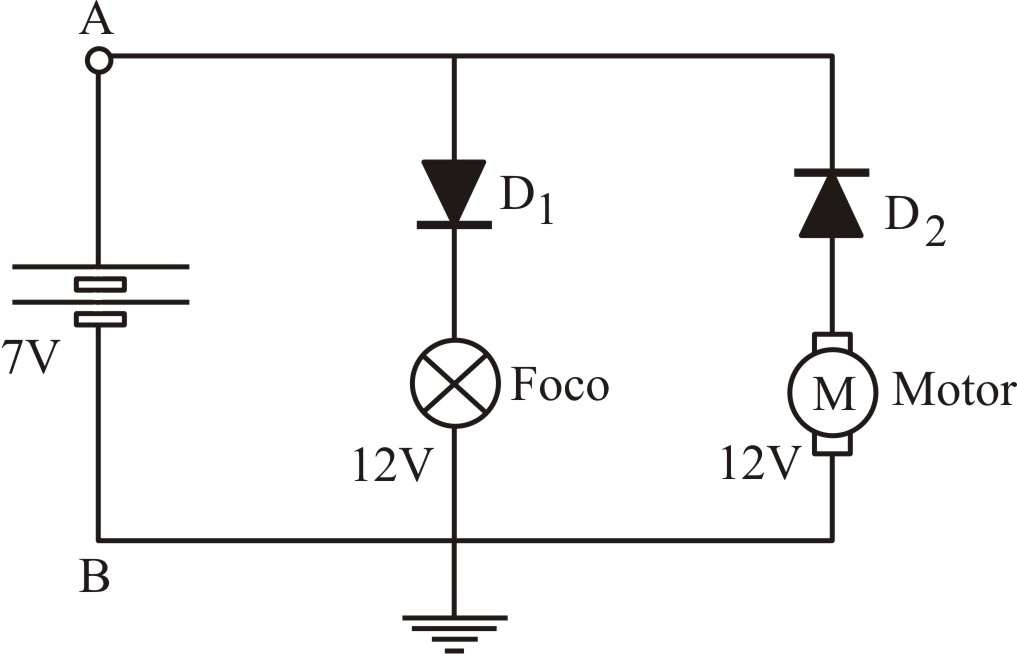
\includegraphics[width=0.46\textwidth]{image23.png}
    \caption{Configuración de diodos $D_1$ y $D_2$.}
    \label{fig:conf-diodos}
\end{figure}

\begin{table}[H]
    \centering
    \caption{Datos de las dos configuraciones de diodos $D_1$ y $D_2$.}
    \label{tab:conf}
    \small
    \renewcommand{\arraystretch}{1.35}
    \begin{tabular}{|>{\centering\arraybackslash}m{2.2cm}|>{\centering\arraybackslash}m{1.9cm}
                    |>{\centering\arraybackslash}m{2.1cm}|>{\centering\arraybackslash}m{2.1cm}
                    |>{\centering\arraybackslash}m{2.1cm}|>{\centering\arraybackslash}m{2.1cm}|}
    \hline
    \multirow{2}{*}{\textbf{Lectura}}
      & \multirow{2}{1.9cm}{\centering\textbf{Voltaje de la fuente}}
      & \multicolumn{4}{c|}{\textbf{EXPERIMENTADO}}\\
    \cline{3-6}
      & & \textbf{Voltaje en el diodo (1)} & \textbf{Voltaje en el foco}
        & \textbf{Voltaje en el diodo (2)} & \textbf{Voltaje en el motor}\\
    \hline
    \multirow{7}{*}{\textbf{Conexión AB}}
       & 1,0 & & & & \\ \cline{2-6}
     & 2,0 & & & & \\ \cline{2-6}
     & 3,0 & & & & \\ \cline{2-6}
     & 4,0 & & & & \\ \cline{2-6}
     & 5,0 & & & & \\ \cline{2-6}
     & 6,0 & & & & \\ \cline{2-6}
     & 7,0 & & & & \\
    \hline
    \multirow{7}{*}{\textbf{Conexión BA}}
       & 1,0 & & & & \\ \cline{2-6}
     & 2,0 & & & & \\ \cline{2-6}
     & 3,0 & & & & \\ \cline{2-6}
     & 4,0 & & & & \\ \cline{2-6}
     & 5,0 & & & & \\ \cline{2-6}
     & 6,0 & & & & \\ \cline{2-6}
     & 7,0 & & & & \\
    \hline
    \end{tabular}
\end{table}

\begin{enumerate}[resume*=confdiodos]
\item Conteste las siguientes preguntas:
\end{enumerate}

\begin{enumerate}[label=\arabic*., leftmargin=2em]
    \item Al hacer la conexión del punto 2: ¿qué sucede? ¿Por qué?
    \item Al hacer la conexión del punto 3: ¿qué sucede? ¿Por qué?
    \item ¿El voltaje del diodo $D_1$ es positivo o negativo? ¿Por qué?
    \item ¿El voltaje del diodo $D_2$ es positivo o negativo? ¿Por qué?
    \item ¿A medida que aumenta el voltaje de la fuente, qué sucede con el LED y con el motor en
          ambas conexiones?
\end{enumerate}

\FloatBarrier
%=======================================================================
\section{El diodo como capacitor variable}
\label{sec:varicap}
%=======================================================================
% Seccion anadida a la guia original. Los datos de la figura del Bode salen
% de LAB2.DAT (barrido en alterna exportado por el simulador) y se trazan con
% herramientas/graficar_bode.py.

% \ref a una subseccion solo imprime su numero (\thesubsection es \arabic), asi
% que aqui se la nombra: un "seccion 2" a secas no le diria nada al alumno.
En el apartado \emph{Polarización inversa} (\ref{sec:inversa}) se comprobó que un diodo
polarizado inversamente apenas conduce. Sin embargo, no se comporta como un circuito abierto: al ensancharse
la zona de deplexión, esta actúa como el dieléctrico entre dos placas conductoras y
el diodo presenta una \emph{capacitancia de juntura} $C_j$ que \textbf{disminuye al
aumentar la tensión inversa}. Un diodo usado de esta forma se denomina
\emph{varicap} o \emph{varactor}.

Si esa capacitancia se conecta a una bobina se obtiene un circuito resonante cuya
frecuencia central puede ajustarse con una tensión continua. Es el principio con el
que sintonizan los receptores de radio.

\subsection{Circuito propuesto}

Arme el circuito de la figura~\ref{fig:resonador}, primero en el simulador y después en
el protoboard.

\begin{figure}[H]
    \centering
    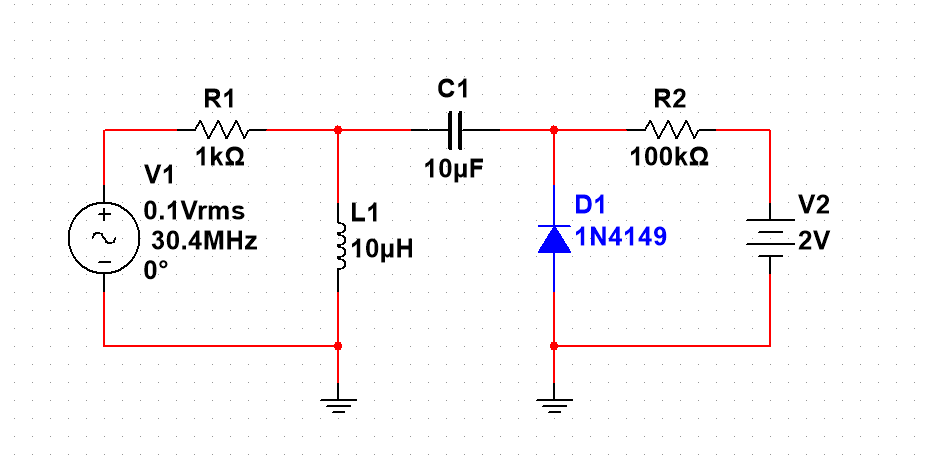
\includegraphics[width=0.80\textwidth]{circuito_resonador.png}
    \caption{Resonador $LC$ sintonizado por la capacitancia de juntura del diodo $D_1$
             en polarización inversa.}
    \label{fig:resonador}
\end{figure}

\noindent Cada componente cumple una función precisa:

\begin{itemize}
    \item $V_2 = \qty{2}{\volt}$ polariza \textbf{inversamente} a $D_1$ a través de
          $R_2 = \qty{100}{\kilo\ohm}$. El valor alto de $R_2$ inyecta la continua sin
          cargar el circuito resonante.
    \item $C_1 = \qty{10}{\micro\farad}$ acopla la señal y bloquea la continua, de modo
          que la polarización de $D_1$ no se pierda por la fuente $V_1$.
    \item $L_1 = \qty{10}{\micro\henry}$ resuena con la capacitancia $C_j$ del diodo.
    \item $R_1 = \qty{1}{\kilo\ohm}$ fija el factor de calidad del conjunto.
    \item $V_1$ entrega \qty{0.1}{\volt} eficaces, una amplitud deliberadamente pequeña:
          si fuese grande, $D_1$ conduciría en los picos y dejaría de portarse como
          capacitor.
\end{itemize}

\FloatBarrier
%-----------------------------------------------------------------------
% \texorpdfstring evita el aviso de hyperref al meter el titulo en los marcadores
% del PDF, donde no se admite modo matematico.
\subsection{Construcción del inductor \texorpdfstring{$L_1$}{L1}}
\label{sec:bobina}
%-----------------------------------------------------------------------
% Apartado nuevo. El inductor de 10 uH no se compra: se bobina. Se usa un
% solenoide de una capa con nucleo de aire, cuyo valor sale de la geometria y
% se puede calcular de antemano; ese es justamente el ejercicio.

$L_1$ es el único componente de la práctica que no se compra hecho: se bobina. Un
solenoide de una sola capa con núcleo de aire tiene la virtud de que su inductancia
queda fijada por la pura geometría --- diámetro, longitud y número de vueltas ---, sin
depender de ningún material magnético. Eso permite calcular la bobina antes de dar la
primera vuelta.

\subsubsection*{La fórmula}

Para una bobina de una capa se emplea la fórmula de Wheeler, aquí con las longitudes
en milímetros:

\begin{equation}
    L\,[\unit{\micro\henry}] = \frac{0.03937\; r^{2} N^{2}}{9\,r + 10\,\ell}
    \label{eq:wheeler}
\end{equation}

\noindent donde $N$ es el número de vueltas, $r$ el \emph{radio medio} del bobinado (el
del formador más el grosor del alambre) y $\ell$ la longitud que ocupa el bobinado.
La expresión es exacta dentro del \qty{1}{\percent} mientras la bobina sea más larga
que \num{0.4} diámetros, condición que el diseño de abajo cumple con holgura.

\subsubsection*{El cálculo}

Se parte de dos decisiones de construcción: un formador de \qty{10}{\milli\metre} de
diámetro y alambre esmaltado AWG~24, que mide \qty{0.51}{\milli\metre} de cobre y unos
\qty{0.57}{\milli\metre} con el esmalte. Bobinando las vueltas \emph{juntas}, cada una
avanza ese paso $p$, de modo que las tres incógnitas se reducen a una sola:

\begin{equation}
    \ell = p\,N = 0.57\,N
    \qquad\qquad
    r = \frac{\qty{10}{\milli\metre} + \qty{0.57}{\milli\metre}}{2} = \qty{5.29}{\milli\metre}
    \label{eq:geometria}
\end{equation}

\noindent Sustituyendo ambas en la ecuación~\eqref{eq:wheeler} e imponiendo
$L_1 = \qty{10}{\micro\henry}$:

\begin{equation*}
    10 = \frac{0.03937 \cdot (5.29)^{2} \cdot N^{2}}{9 (5.29) + 10 (0.57\,N)}
       = \frac{1.102\,N^{2}}{47.6 + 5.70\,N}
\end{equation*}

\noindent que reordenada es una simple ecuación de segundo grado en $N$:

\begin{equation*}
    1.102\,N^{2} - 57.0\,N - 476 = 0
    \qquad\Longrightarrow\qquad
    N = \frac{57.0 + \sqrt{57.0^{2} + 4(1.102)(476)}}{2(1.102)} = 59.0
\end{equation*}

\noindent Son, pues, \textbf{59 vueltas}, que ocupan $\ell = 0.57 \times 59 =
\qty{33.6}{\milli\metre}$. La bobina resulta \num{3.2} veces más larga que ancha, dentro
del rango de validez de Wheeler. El alambre que hay que cortar es el perímetro medio por
el número de vueltas, más un margen para las puntas:

\begin{equation*}
    \text{longitud} = N \pi d_{\text{medio}} + 2 (\qty{100}{\milli\metre})
                    = 59 \pi (\qty{10.57}{\milli\metre}) + \qty{200}{\milli\metre}
                    \approx \qty{2.2}{\metre}
\end{equation*}

\begin{table}[H]
    \centering
    \caption{Resumen del diseño de $L_1$: solenoide de una capa con núcleo de aire.}
    \label{tab:bobina}
    \small
    \renewcommand{\arraystretch}{1.35}
    \begin{tabular}{|>{\raggedright\arraybackslash}m{6.4cm}
                    |>{\centering\arraybackslash}m{1.8cm}
                    |>{\centering\arraybackslash}m{3.6cm}|}
    \hline
    \textbf{Parámetro} & \textbf{Símbolo} & \textbf{Valor}\\
    \hline
    Diámetro del formador          & $d$    & \qty{10}{\milli\metre} \\ \hline
    Calibre del alambre            & ---    & AWG 24 (\qty{0.51}{\milli\metre}) \\ \hline
    Paso entre vueltas, con esmalte& $p$    & \qty{0.57}{\milli\metre} \\ \hline
    Radio medio del bobinado       & $r$    & \qty{5.29}{\milli\metre} \\ \hline
    Número de vueltas              & $N$    & 59 \\ \hline
    Longitud del bobinado          & $\ell$ & \qty{33.6}{\milli\metre} \\ \hline
    Alambre necesario              & ---    & \qty{2.2}{\metre} \\ \hline
    Inductancia resultante         & $L_1$  & \qty{10.0}{\micro\henry} \\ \hline
    \end{tabular}
\end{table}

\subsubsection*{Por qué AWG 24}

El calibre no se elige aquí por la corriente, que es de apenas unos microamperios, sino
por dos razones distintas. La primera es mecánica: el AWG~24 es lo bastante rígido para
que la bobina se sostenga sola al retirar el formador y no cambie de forma --- y con
ella de inductancia --- al manipularla.

La segunda es el \textbf{efecto pelicular}. A frecuencias altas la corriente no ocupa
toda la sección del conductor, sino una capa superficial de espesor

\begin{equation}
    \delta\,[\unit{\milli\metre}] = \frac{66}{\sqrt{f\,[\unit{\hertz}]}}
    \qquad\text{que en cobre y a \qty{30}{\mega\hertz} vale}\qquad
    \delta \approx \qty{12}{\micro\metre}
    \label{eq:pelicular}
\end{equation}

\noindent Es decir: de los \qty{255}{\micro\metre} de radio que tiene el AWG~24, solo los
\num{12} más externos conducen. Engrosar el alambre no añade cobre útil en proporción a
su sección, sino a su \emph{perímetro}, y por eso pasar a un calibre mucho mayor apenas
mejora las pérdidas mientras estorba el bobinado. Un calibre bastante más fino, en
cambio, sí las empeora y además no se sostiene. El AWG~24 es el punto de equilibrio; el
AWG~22 y el AWG~26 también sirven, recalculando $p$ y por tanto $N$.

\subsubsection*{Verificación}

Como el valor depende de lo apretado que quede el bobinado, hay que comprobarlo. Mida la
longitud real $\ell$ del solenoide terminado y vuelva a evaluar la
ecuación~\eqref{eq:wheeler} con ella. Después contrástelo por resonancia, que es una
medida y no una estimación: conecte en paralelo con la bobina el condensador cerámico de
\qty{1}{\nano\farad}, haga un barrido en alterna y localice el pico. De la frecuencia
medida se despeja la inductancia:

\begin{equation}
    L_1 = \frac{1}{\left(2\pi f_0\right)^{2} C}
    \qquad\text{con \qty{1}{\nano\farad} y \qty{10}{\micro\henry} se espera}\qquad
    f_0 \approx \qty{1.59}{\mega\hertz}
    \label{eq:verificacion}
\end{equation}

\noindent Una diferencia de un \qtyrange{5}{10}{\percent} respecto de los
\qty{10}{\micro\henry} es normal y no invalida nada: basta con anotar el valor real
medido y usar \emph{ese} en los cálculos de la tabla~\ref{tab:resonador}, no el nominal.

\FloatBarrier
\subsection{Procedimiento}

\begin{enumerate}[label=\textbf{\alph*)}, leftmargin=*, labelsep=0.6em]
\item Ejecute un análisis en alterna (\emph{AC sweep}) sobre el nodo marcado como
\texttt{C1(2)}, entre \qty{100}{\kilo\hertz} y \qty{1}{\giga\hertz}, con al menos
10 puntos por década y el eje vertical en decibelios.

\item Exporte el resultado a un archivo de texto. El archivo \texttt{LAB2.DAT} que
acompaña a esta guía es una exportación de ese mismo barrido y sirve como referencia.

\item Grafique la curva con Python, como se pide también en la
sección~\ref{sec:analisis}. El resultado debe parecerse al de la
figura~\ref{fig:bode}.

% El barrido en alterna de este circuito cae por encima de los 30 MHz, fuera del
% alcance del instrumental del laboratorio: sobre el montaje real se comprueba la
% polarizacion continua, que es lo que si se puede medir con el multimetro.
\item Sobre el circuito montado en el protoboard, mida con el multímetro la tensión
continua entre el ánodo y el cátodo de $D_1$ y confirme que está polarizado
inversamente con los \qty{2}{\volt} que entrega $V_2$. Verifique también que por
$R_2$ prácticamente no circula corriente, que es la señal de que el diodo se
comporta como el capacitor que este apartado estudia y no como un conductor.
\end{enumerate}

\begin{figure}[H]
    \centering
    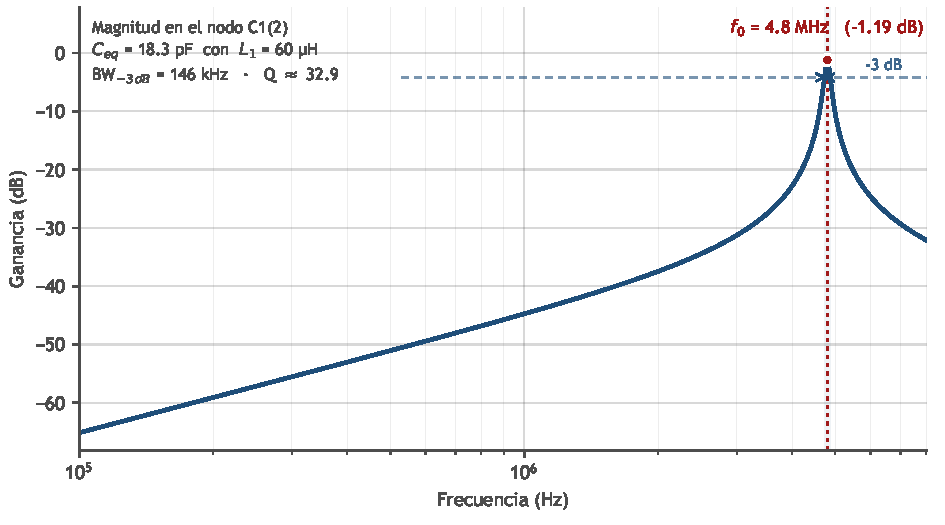
\includegraphics[width=\textwidth]{bode_resonador.pdf}
    \caption{Diagrama de Bode (magnitud) del resonador, trazado a partir de
             \texttt{LAB2.DAT}. Por debajo de $f_0$ la respuesta sube a
             \qty{20}{\decibel} por década porque domina la reactancia de $L_1$; por
             encima cae a igual ritmo porque domina la de $C_j$.}
    \label{fig:bode}
\end{figure}

\begin{notatec}{qué se puede y qué no se puede leer en estos datos}
El barrido tiene 10 puntos por década, suficiente para situar el pico pero no para
resolverlo con finura: el ancho de banda y el factor $Q$ que se obtengan de él son
estimaciones. Además, las once columnas que exporta \texttt{LAB2.DAT} son idénticas
entre sí, de modo que el parámetro del barrido no llegó a afectar al circuito; para
estudiar cómo cambia $f_0$ con la tensión inversa hay que repetir la simulación
variando $V_2$ a mano, tal como pide la tabla~\ref{tab:resonador}.
\end{notatec}

\FloatBarrier
\subsection{Mediciones}

Repita el barrido para cada valor de $V_2$ y complete la tabla~\ref{tab:resonador}.
La capacitancia se despeja de la frecuencia de resonancia:

\begin{equation}
    f_0 = \frac{1}{2\pi\sqrt{L_1\,C_j}}
    \qquad\Longrightarrow\qquad
    C_j = \frac{1}{\left(2\pi f_0\right)^2 L_1}
    \label{eq:resonancia}
\end{equation}

\begin{table}[H]
    \centering
    \caption{Frecuencia de resonancia del tanque en función de la tensión inversa
             aplicada al diodo.}
    \label{tab:resonador}
    \small
    \renewcommand{\arraystretch}{1.35}
    \begin{tabular}{|>{\centering\arraybackslash}m{2.6cm}|>{\centering\arraybackslash}m{2.8cm}
                    |>{\centering\arraybackslash}m{2.8cm}|>{\centering\arraybackslash}m{3.4cm}|}
    \hline
    \textbf{Tensión inversa} ($V_2$) & \textbf{Frecuencia de resonancia} ($f_0$)
      & \textbf{Ganancia en el pico} & \textbf{Capacitancia del diodo} ($C_j$)\\
    \hline
    \qty{0}{\volt}  & & & \\ \hline
    \qty{1}{\volt}  & & & \\ \hline
    \qty{2}{\volt}  & & & \\ \hline
    \qty{5}{\volt}  & & & \\ \hline
    \qty{10}{\volt} & & & \\ \hline
    \end{tabular}
\end{table}

\subsection{Preguntas}

\begin{enumerate}[label=\arabic*., leftmargin=2em]
    \item A partir de la figura~\ref{fig:bode} y de la ecuación~\eqref{eq:resonancia},
          calcule la capacitancia que presenta $D_1$ con $V_2 = \qty{2}{\volt}$.
          Compárela con la que indica la hoja de datos del 1N4149.
    \item La fuente $V_1$ está fijada en \qty{30.4}{\mega\hertz}, pero el pico de la
          simulación no cae exactamente ahí. ¿A qué se debe la diferencia y qué
          capacitancia haría que ambas coincidieran?
    \item Según los valores que anotó en la tabla~\ref{tab:resonador}, ¿la frecuencia
          de resonancia sube o baja al aumentar $V_2$? Explíquelo a partir del ancho de
          la zona de deplexión.
    \item ¿Qué ocurriría si $V_1$ entregase \qty{5}{\volt} eficaces en lugar de
          \qty{0.1}{\volt}? ¿Seguiría siendo válido el análisis?
    \item ¿Por qué se emplea aquí un 1N4149 y no el 1N4007 de las secciones
          anteriores? Compare el tiempo de recuperación inversa de ambos.
\end{enumerate}

\FloatBarrier
%=======================================================================
\section{Análisis de resultados \puntos{4}}
\label{sec:analisis}
%=======================================================================
\begin{itemize}
    \item Realice una gráfica $V_D$ \emph{vs.} $I_D$ con las medidas anotadas en las
          tablas~\ref{tab:directa} y~\ref{tab:inversa} (simulación y medición). Esta gráfica
          deberá ser generada con Python. Identificar las regiones de la curva característica del
          diodo semiconductor.
\end{itemize}

%=======================================================================
\section{Cuestionario \puntos{2}}
%=======================================================================
\begin{enumerate}
    \item ¿A partir de qué voltaje comienza a conducir el diodo?
    \item ¿Por qué la corriente aumenta rápidamente después del voltaje umbral?
    \item ¿Qué diferencias observa entre la simulación y el experimento?
    \item ¿Qué ocurre cuando el diodo se polariza inversamente?
    \item ¿Por qué la corriente inversa es muy pequeña?
\end{enumerate}

%=======================================================================
\section{Conclusiones \puntos{2}}
%=======================================================================
\begin{itemize}
    \item Deberán consignar 05 conclusiones como mínimo.
\end{itemize}

\end{document}
